\documentclass[border=10pt]{standalone}
% Shared style for the EMONI diagrams. Build: tectonic <file>.tex, then pdftocairo -svg.
\usepackage{fontspec}
\setmainfont{FiraSans}[Extension=.otf,UprightFont=*-Regular,BoldFont=*-SemiBold,ItalicFont=*-Italic,BoldItalicFont=*-SemiBoldItalic]
\setmonofont{FiraMono}[Extension=.otf,UprightFont=*-Regular,BoldFont=*-Medium,Scale=0.9]
\usepackage{tikz}
\usetikzlibrary{arrows.meta,positioning,shapes.geometric,shapes.misc,calc,fit,backgrounds}
\definecolor{eg}{HTML}{11903B}   % EMONI green
\definecolor{egl}{HTML}{E8F7EE}
\definecolor{eb}{HTML}{2A78D6}   % blue
\definecolor{ebl}{HTML}{EAF2FC}
\definecolor{eo}{HTML}{D9631E}   % orange
\definecolor{eol}{HTML}{FDF0E7}
\definecolor{ep}{HTML}{7C4DCC}   % purple
\definecolor{epl}{HTML}{F2ECFB}
\definecolor{er}{HTML}{C5221F}   % red
\definecolor{erl}{HTML}{FCEAEA}
\definecolor{ink}{HTML}{1F2328}
\definecolor{mute}{HTML}{59636E}
\definecolor{line}{HTML}{D0D7DE}
\tikzset{
  every node/.style={text=ink,font=\small},
  >={Stealth[length=2.4mm]},
  % sequence diagrams
  life/.style={draw=line,dashed,thick},
  head/.style={draw=#1,fill=#1!8,rounded corners=3pt,minimum width=27mm,minimum height=11mm,align=center,font=\small\bfseries,thick},
  act/.style={draw=#1,fill=#1!18,minimum width=2.2mm},
  msg/.style={->,thick,draw=ink},
  ret/.style={->,dashed,draw=mute},
  mlabel/.style={font=\footnotesize,fill=white,inner sep=1.5pt,align=center},
  note/.style={draw=#1,fill=#1!8,rounded corners=2pt,font=\footnotesize,align=left,inner sep=4pt},
  frag/.style={draw=mute,rounded corners=2pt},
  fraglabel/.style={draw=mute,fill=white,font=\footnotesize\bfseries,inner sep=2.5pt,anchor=north west},
  % activity diagrams
  start/.style={circle,fill=ink,minimum size=4mm,inner sep=0},
  stop/.style={circle,draw=ink,thick,minimum size=5mm,inner sep=0,path picture={\fill[ink] (path picture bounding box.center) circle (1.4mm);}},
  step/.style={draw=#1,fill=#1!8,rounded corners=5pt,thick,minimum height=9mm,minimum width=40mm,align=center,font=\small},
  step/.default=eg,
  dec/.style={diamond,aspect=2.2,draw=ink,fill=white,thick,inner sep=1.5pt,align=center,font=\footnotesize},
  flow/.style={->,thick,draw=ink},
  guard/.style={font=\footnotesize\itshape,text=mute,fill=white,inner sep=1.5pt},
  lane/.style={draw=line,fill=#1,rounded corners=4pt},
  lanetitle/.style={font=\small\bfseries,text=mute},
}

% The sleep-current leak found on the bench, drawn generically: an external pull-up against an internal pull-down.
\begin{document}
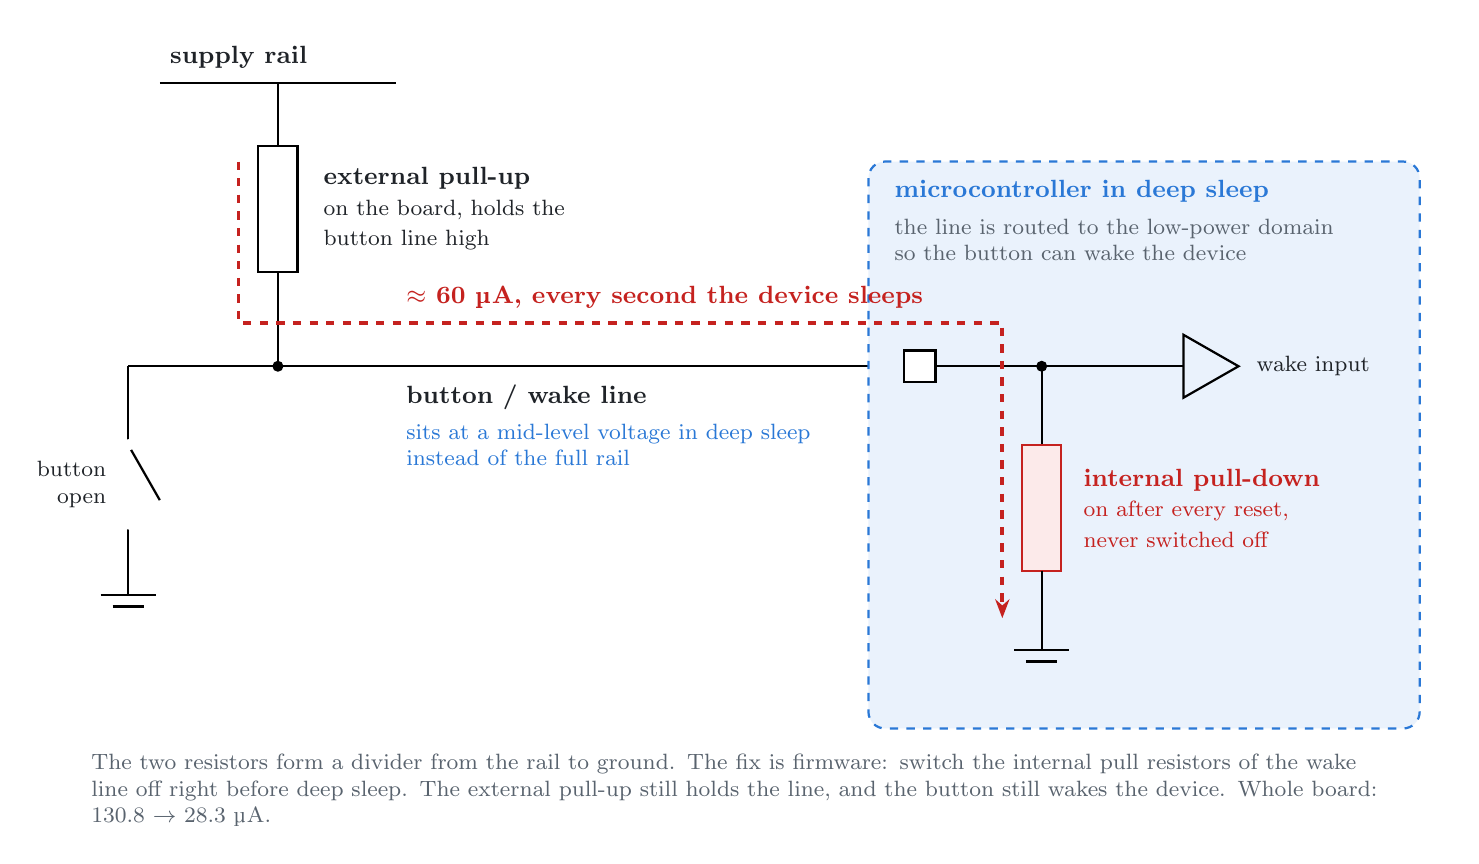
\begin{tikzpicture}[x=1cm,y=1cm,thick]
\fill[white] (-1.2,1.3) rectangle (16.4,-8.6);
\draw (0,0.6) -- (3,0.6); \node[anchor=south west,font=\small\bfseries] at (0,0.65) {supply rail};
\draw (1.5,0.6) -- (1.5,-0.2);
\draw[fill=white] (1.25,-0.2) rectangle (1.75,-1.8);
\node[anchor=west,align=left] at (1.95,-1.0) {\textbf{external pull-up}\\{\footnotesize on the board, holds the}\\{\footnotesize button line high}};
\draw (1.5,-1.8) -- (1.5,-3.0);
\fill (1.5,-3.0) circle (0.07);
\draw (-0.4,-3.0) -- (9.6,-3.0);
\node[anchor=north west,font=\small\bfseries] at (3.0,-3.1) {button / wake line};
\node[anchor=north west,text=eb,align=left,font=\footnotesize] at (3.0,-3.6) {sits at a mid-level voltage in deep sleep\\instead of the full rail};
\draw (-0.4,-3.0) -- (-0.4,-4.0); \draw (-0.4,-4.0) -- (0.0,-4.7); \draw (-0.4,-5.0) -- (-0.4,-5.9);
\fill[white,draw] (-0.4,-4.0) circle (0.06); \fill[white,draw] (-0.4,-5.0) circle (0.06);
\node[anchor=east,align=right,font=\footnotesize] at (-0.55,-4.5) {button\\open};
\draw (-0.75,-5.9) -- (-0.05,-5.9); \draw (-0.6,-6.05) -- (-0.2,-6.05);
% MCU box
\draw[eb,dashed,fill=ebl,rounded corners=6pt] (9.0,-0.4) rectangle (16.0,-7.6);
\node[anchor=north west,text=eb,font=\small\bfseries,align=left] at (9.2,-0.5) {microcontroller in deep sleep};
\node[anchor=north west,text=mute,font=\footnotesize,align=left] at (9.2,-1.0) {the line is routed to the low-power domain\\so the button can wake the device};
\draw[fill=white] (9.45,-2.8) rectangle (9.85,-3.2);
\draw (9.85,-3.0) -- (13.0,-3.0); \fill (11.2,-3.0) circle (0.07);
\draw (11.2,-3.0) -- (11.2,-4.0);
\draw[er,fill=erl] (10.95,-4.0) rectangle (11.45,-5.6);
\node[anchor=west,text=er,align=left] at (11.6,-4.8) {\textbf{internal pull-down}\\{\footnotesize on after every reset,}\\{\footnotesize never switched off}};
\draw (11.2,-5.6) -- (11.2,-6.6); \draw (10.85,-6.6) -- (11.55,-6.6); \draw (11.0,-6.75) -- (11.4,-6.75);
\draw (13.0,-2.6) -- (13.0,-3.4) -- (13.7,-3.0) -- cycle; \node[anchor=west,font=\footnotesize] at (13.8,-3.0) {wake input};
% current path
\draw[er,dashed,->,line width=1.4pt] (1.0,-0.4) -- (1.0,-2.45) -- (10.7,-2.45) -- (10.7,-6.2);
\node[text=er,font=\small\bfseries,anchor=south west] at (3.0,-2.4) {$\approx$ 60 \textmu A, every second the device sleeps};
\node[anchor=north west,align=left,font=\footnotesize,text=mute,text width=16.6cm] at (-1.0,-7.8) {The two resistors form a divider from the rail to ground. The fix is firmware: switch the internal pull resistors of the wake line off right before deep sleep. The external pull-up still holds the line, and the button still wakes the device. Whole board: 130.8 $\rightarrow$ 28.3 \textmu A.};
\end{tikzpicture}
\end{document}
